\newcommand{\IDWConfidencePlot}{%
\begin{figure}[H]
\centering
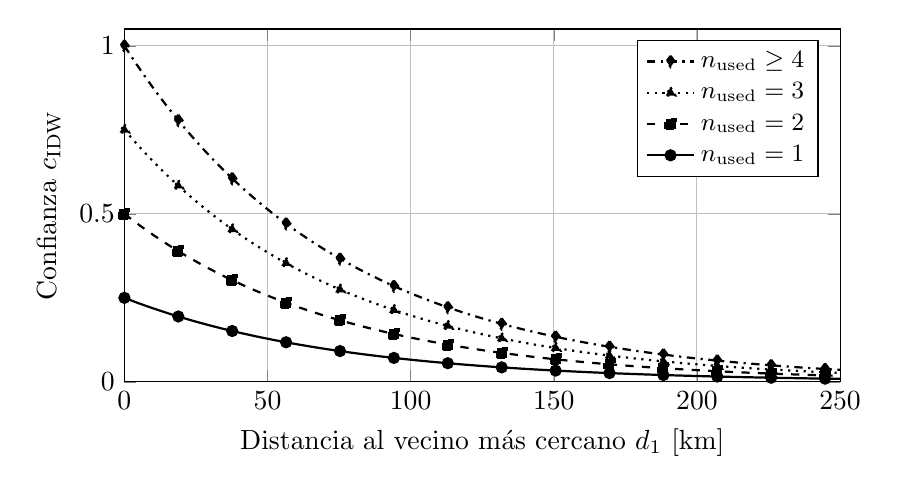
\begin{tikzpicture}
\begin{axis}[
    width=0.88\textwidth,
    height=0.50\textwidth,
    xlabel={Distancia al vecino más cercano \(d_1\) [km]},
    ylabel={Confianza \(c_{\mathrm{IDW}}\)},
    xmin=0, xmax=250,
    ymin=0, ymax=1.05,
    domain=0:250,
    samples=240,
    grid=both,
    legend style={at={(0.97,0.97)}, anchor=north east, font=\small},
    reverse legend,
    every axis plot/.append style={thick}
]

\addplot[
    mark=*,
    mark size=1.8pt,
    mark repeat=18
] {min(1/4,1)*exp(-x/75)};
\addlegendentry{\(n_{\mathrm{used}}=1\)}

\addplot[
    dashed,
    mark=square*,
    mark size=1.8pt,
    mark repeat=18
] {min(2/4,1)*exp(-x/75)};
\addlegendentry{\(n_{\mathrm{used}}=2\)}

\addplot[
    dotted,
    mark=triangle*,
    mark size=2pt,
    mark repeat=18
] {min(3/4,1)*exp(-x/75)};
\addlegendentry{\(n_{\mathrm{used}}=3\)}

\addplot[
    dash dot,
    mark=diamond*,
    mark size=2pt,
    mark repeat=18
] {min(4/4,1)*exp(-x/75)};
\addlegendentry{\(n_{\mathrm{used}}\geq 4\)}

\end{axis}
\end{tikzpicture}
\caption{Decaimiento de la confianza del relleno IDW en función de la distancia al vecino más cercano, para distintos números de estaciones vecinas efectivamente usadas para la configuración actual.}
\label{fig:idw_conf_vs_distance}
\end{figure}%
}

\newcommand{\TempConfidencePlot}{%
\begin{figure}[H]
\centering
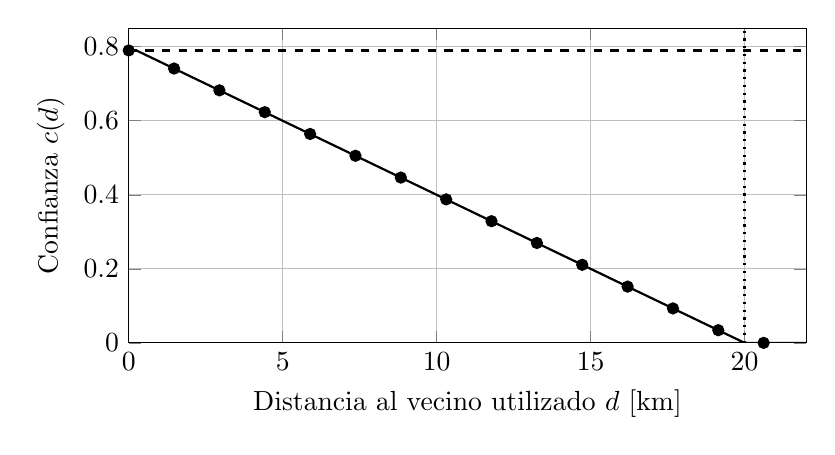
\begin{tikzpicture}
\begin{axis}[
    width=0.84\textwidth,
    height=0.46\textwidth,
    xlabel={Distancia al vecino utilizado \(d\) [km]},
    ylabel={Confianza \(c(d)\)},
    xmin=0, xmax=22,
    ymin=0, ymax=0.85,
    domain=0:22,
    samples=240,
    grid=both,
    legend style={at={(0.97,0.97)}, anchor=north east, font=\small},
    every axis plot/.append style={thick}
]

% Curva principal
\addplot[
    mark=*,
    mark size=1.8pt,
    mark repeat=16
] {max(0,min(0.79,0.8*(1 - x/20)))};

% Línea horizontal en 0.79
\addplot[dashed] coordinates {(0,0.79) (22,0.79)};

% Línea vertical en 20 km
\addplot[dotted] coordinates {(20,0) (20,0.85)};

\end{axis}
\end{tikzpicture}
\caption{Decaimiento lineal de la confianza del relleno por vecindad en temperatura en función de la distancia al vecino utilizado para la configuración actual.}
\label{fig:temp_conf_vs_distance}
\end{figure}%
}

\newcommand{\LSCDFThresholdSeparationPlot}{%
\begin{figure}[H]
\centering
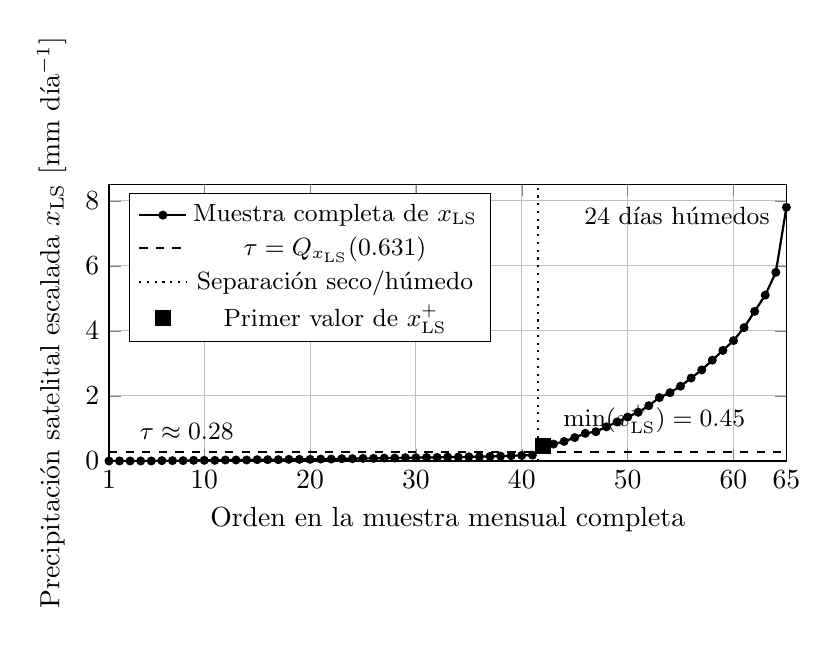
\begin{tikzpicture}
\begin{axis}[
    width=0.84\textwidth,
    height=0.42\textwidth,
    xlabel={Orden en la muestra mensual completa},
    ylabel={Precipitación satelital escalada \(x_{\mathrm{LS}}\) [mm día\(^{-1}\)]},
    xmin=1, xmax=65,
    ymin=0, ymax=8.5,
    xtick={1,10,20,30,40,50,60,65},
    grid=both,
    legend style={at={(0.03,0.97)}, anchor=north west, font=\small},
    every axis plot/.append style={thick}
]

\addplot[
    mark=*,
    mark size=1.2pt
] coordinates {
(1,0.00) (2,0.00) (3,0.00) (4,0.00) (5,0.00)
(6,0.01) (7,0.01) (8,0.01) (9,0.02) (10,0.02)
(11,0.02) (12,0.03) (13,0.03) (14,0.03) (15,0.04)
(16,0.04) (17,0.04) (18,0.05) (19,0.05) (20,0.05)
(21,0.06) (22,0.06) (23,0.07) (24,0.07) (25,0.08)
(26,0.08) (27,0.09) (28,0.09) (29,0.10) (30,0.10)
(31,0.11) (32,0.11) (33,0.12) (34,0.12) (35,0.13)
(36,0.13) (37,0.14) (38,0.15) (39,0.16) (40,0.17)
(41,0.18) (42,0.45) (43,0.52) (44,0.60) (45,0.72)
(46,0.85) (47,0.90) (48,1.05) (49,1.20) (50,1.35)
(51,1.50) (52,1.70) (53,1.95) (54,2.10) (55,2.30)
(56,2.55) (57,2.80) (58,3.10) (59,3.40) (60,3.70)
(61,4.10) (62,4.60) (63,5.10) (64,5.80) (65,7.80)
};
\addlegendentry{Muestra completa de \(x_{\mathrm{LS}}\)}

\addplot[dashed] coordinates {(1,0.28) (65,0.28)};
\addlegendentry{\(\tau = Q_{x_{\mathrm{LS}}}(0.631)\)}

\addplot[dotted] coordinates {(41.5,0) (41.5,8.5)};
\addlegendentry{Separación seco/húmedo}

\addplot[
    only marks,
    mark=square*,
    mark size=2.5pt
] coordinates {(42,0.45)};
\addlegendentry{Primer valor de \(x_{\mathrm{LS}}^{+}\)}

\node[font=\small, anchor=south west] at (axis cs:3,0.36)
{\(\tau \approx 0.28\)};

\node[font=\small, anchor=south west] at (axis cs:43,0.55)
{\(\min(x_{\mathrm{LS}}^{+})=0.45\)};

\node[font=\small, anchor=north west] at (axis cs:5,8.1)
{41 días secos};

\node[font=\small, anchor=north west] at (axis cs:45,8.1)
{24 días húmedos};

\end{axis}
\end{tikzpicture}
\caption{Separación entre la muestra mensual completa \(x_{\mathrm{LS}}\) y la submuestra húmeda \(x_{\mathrm{LS}}^{+}\). La muestra contiene \(65\) pares válidos después de aplicar el filtro de confianza \(\texttt{conf\_interp} \geq \texttt{ref\_min\_conf}=0.9\). El umbral \(\tau\) se calcula sobre la muestra completa, no sobre la submuestra húmeda. En este ejemplo, \(\tau \approx 0.28\) mm día\(^{-1}\), mientras que el menor valor que entra al CDF matching es \(0.45\) mm día\(^{-1}\).}
\label{fig:lscdf_threshold_separation}
\end{figure}%
}

\newcommand{\LSCDFQuantileMappingPlot}{%
\begin{figure}[H]
\centering
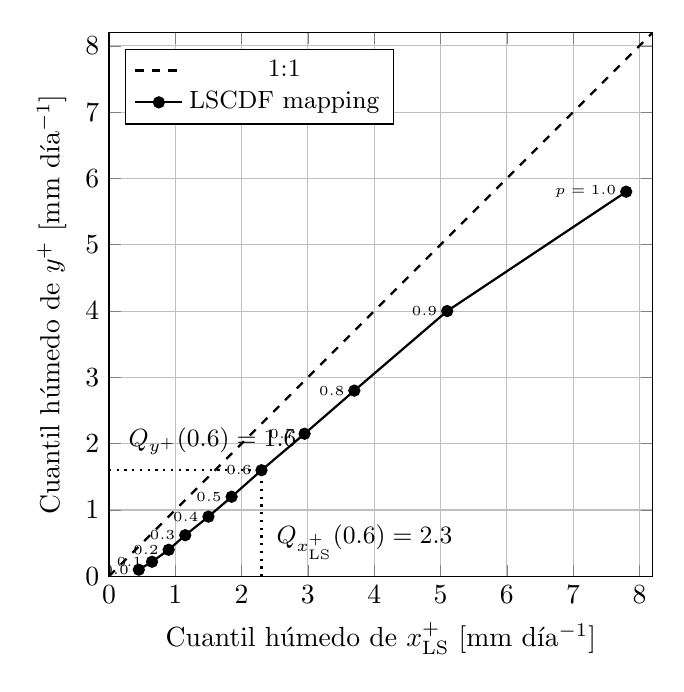
\begin{tikzpicture}
\begin{axis}[
    width=0.70\textwidth,
    height=0.70\textwidth,
    axis equal image,
    xlabel={Cuantil húmedo de \(x_{\mathrm{LS}}^{+}\) [mm día\(^{-1}\)]},
    ylabel={Cuantil húmedo de \(y^{+}\) [mm día\(^{-1}\)]},
    xmin=0, xmax=8.2,
    ymin=0, ymax=8.2,
    xtick={0,1,2,3,4,5,6,7,8},
    ytick={0,1,2,3,4,5,6,7,8},
    grid=both,
    legend style={at={(0.03,0.97)}, anchor=north west, font=\small},
    every axis plot/.append style={thick}
]

% Línea 1:1
\addplot[dashed] coordinates {(0,0) (8.2,8.2)};
\addlegendentry{1:1}

% Curva de mapeo uniendo los 11 cuantiles del ejemplo
\addplot[
    mark=*,
    mark size=1.8pt
] coordinates {
    (0.45,0.10)
    (0.65,0.22)
    (0.90,0.40)
    (1.15,0.62)
    (1.50,0.90)
    (1.85,1.20)
    (2.30,1.60)
    (2.95,2.15)
    (3.70,2.80)
    (5.10,4.00)
    (7.80,5.80)
};
\addlegendentry{LSCDF mapping}

% Etiquetas de p, con distancia fija a la izquierda de cada punto
\node[font=\tiny, anchor=east, xshift=-0.1pt] at (axis cs:0.45,0.10) {\(0.0\)};
\node[font=\tiny, anchor=east, xshift=-0.1pt] at (axis cs:0.65,0.22) {\(0.1\)};
\node[font=\tiny, anchor=east, xshift=-0.1pt] at (axis cs:0.90,0.40) {\(0.2\)};
\node[font=\tiny, anchor=east, xshift=-0.1pt] at (axis cs:1.15,0.62) {\(0.3\)};
\node[font=\tiny, anchor=east, xshift=-0.1pt] at (axis cs:1.50,0.90) {\(0.4\)};
\node[font=\tiny, anchor=east, xshift=-0.1pt] at (axis cs:1.85,1.20) {\(0.5\)};
\node[font=\tiny, anchor=east, xshift=-0.1pt] at (axis cs:2.30,1.60) {\(0.6\)};
\node[font=\tiny, anchor=east, xshift=-0.1pt] at (axis cs:2.95,2.15) {\(0.7\)};
\node[font=\tiny, anchor=east, xshift=-0.1pt] at (axis cs:3.70,2.80) {\(0.8\)};
\node[font=\tiny, anchor=east, xshift=-0.1pt] at (axis cs:5.10,4.00) {\(0.9\)};
\node[font=\tiny, anchor=east, xshift=-0.1pt] at (axis cs:7.80,5.80) {\(p=1.0\)};

% Ejemplo destacado para p = 0.6
\addplot[dotted] coordinates {(2.30,0) (2.30,1.60)};
\addplot[dotted] coordinates {(0,1.60) (2.30,1.60)};

\node[font=\small, anchor=south west] at (axis cs:2.38,0.10)
{\(Q_{x_{\mathrm{LS}}^{+}}(0.6)=2.3\)};

\node[font=\small, anchor=south west] at (axis cs:0.15,1.68)
{\(Q_{y^{+}}(0.6)=1.6\)};

\end{axis}
\end{tikzpicture}
\caption{Mapeo de cuantiles húmedos en el ejemplo LSCDF. La figura muestra \(11\) cuantiles ilustrativos, correspondientes a \(p=0,0.1,\dots,1.0\).}
\label{fig:lscdf_quantile_mapping}
\end{figure}%
}